\documentclass[11pt,a4paper]{article}
\usepackage[T1]{fontenc}
\usepackage[utf8]{inputenc}
\usepackage{lmodern}
\usepackage{amsmath,amssymb,amsthm}
\usepackage{geometry}
\geometry{margin=2.6cm}
\usepackage{graphicx}
\usepackage{booktabs}
\usepackage{array}
\usepackage{enumitem}
\usepackage{float}
\usepackage{rotating}
\usepackage[hidelinks]{hyperref}
\hypersetup{pdftitle={A programmer's walkthrough of inter-universal Teichmuller theory},pdfauthor={Toshihisa Urahigashi}}
\setlist{itemsep=2pt,topsep=4pt}
\raggedbottom

\newcommand{\qq}{\underline{\underline{q}}{}}
\newcommand{\Th}{\underline{\underline{\Theta}}{}}
\newcommand{\F}{\mathbb{F}}
\newcommand{\Q}{\mathbb{Q}}
\newcommand{\Z}{\mathbb{Z}}
\newcommand{\R}{\mathbb{R}}
\newcommand{\cO}{\mathcal{O}}
\newcommand{\cI}{\mathcal{I}}
\newcommand{\ord}{\operatorname{ord}}
\newcommand{\Fmod}{F_{\mathrm{mod}}}
\newcommand{\Vbad}{\mathbb{V}^{\mathrm{bad}}_{\mathrm{mod}}}
\newcommand{\code}[1]{\texttt{#1}}

\title{A programmer's walkthrough of\\ inter-universal Teichm\"uller theory:\\
running the multiradial algorithm\\ on explicit initial $\Theta$-data}
\author{Toshihisa Urahigashi\\\small\texttt{123026.urahigashi.toshihisa@gmail.com}}
\date{Version 1.1.0, 5 November 2026\\\small\href{https://doi.org/10.5281/zenodo.23955994}{doi:10.5281/zenodo.23955994}}

\begin{document}
\maketitle

\begin{abstract}
We describe a program, with an interactive web page, that runs on explicit numbers those operations of
inter-universal Teichm\"uller theory (IUT) that can be written as procedures. Its input is one of seven explicit
initial $\Theta$-data from an earlier catalogue. The program computes the Tate parameters and the local data
$p$-adically, arranges the labels and processions, and keeps the two Hodge theaters of a $\Theta$-link as
copies of the local fields separated by type, so that only a ``cable''---the unit-group data and one unlabelled
value-group object---passes between them, after an analogy that the source itself draws. It then computes
log-shells, Kummer read-outs, the containers of the multiradial representation and the possible images of the
theta values, and evaluates the log-volume of the holomorphic hull of their union, as an exact combination of
logarithms, for three readings of the label indeterminacy and two models of the indeterminacy (Ind2):
multiplication by units, and all $\Z_p$-linear automorphisms of the log-shells of the factors, as in the Lean
formalization lana-agents/iut. For the second model the hull is given by a closed form from the author's earlier
note; it is exact where $p$ is odd and $e\le p-2$, and bracketed elsewhere. Finally it places side by
side the two quantities that Step~(xi) of the proof of Corollary~3.12 of IUT~III compares. In the reading of
IUT~IV the two models give the two forms of the comparison that lana-agents/iut calls the Scholze--Stix inequality
and the variant of Corollary~3.12, and the program computes their difference for each datum; version~1.1.0 adds the
second model. Infinite objects are
computed in finite windows, and the program prints how its output stabilizes as the windows grow. The
properties IPL, SHE and APT of Remark~3.11.1 of IUT~III appear as the shape of the code and as records of its
execution; the inference~(xi-f) is displayed, not evaluated. The purpose is expository. No conclusion is drawn
about Corollary~3.12, Theorem~1.10 of IUT~IV, or the abc conjecture. Turning the objects and processes of IUT
into data types, with IPL and APT proved for a Lean model, has been done earlier and on a broader scale in the
toolkit motizukipdf; the formulas for the containers and the distinction between the readings are taken from the
Lean formalization lana-agents/iut.
\end{abstract}

\section{Introduction}\label{sec:intro}

The four papers on inter-universal Teichm\"uller theory~\cite{IUT1,IUT2,IUT3,IUT4} are long, and much of their
length goes into showing that each operation can be carried out on group-theoretic data alone, without the
ring structures of the objects it acts on, and that the operations are compatible with one another. The
operations themselves can be described as procedures acting on an initial $\Theta$-datum: build labels and
Hodge theaters, compute theta values, pass data through the $\Theta$-link and the log-link, place the theta
values into containers up to certain indeterminacies, take a hull, and compare two log-volumes. The source
itself invites this view. Remark~3.11.1(iv) of~\cite{IUT3} compares the theta functions and theta values used
by the multiradial algorithm to the internal structure of a CPU or an operating system, which matters for how the
algorithm runs but not for an ``end user'' who only feeds it input data and reads its output, and it compares
the prime-strip of the $\Theta$-link to a cable connecting separate computers. Mochizuki's report on the
formalization of IUT~\cite[\S1]{Formal} describes formalization as a tool for communicating the logical
structure of the theory, rather than mainly as a tool for verification, and its overview~\cite[\S3]{Formal} states
the main point in terms that a programmer can take literally: the multiplicative monoid structures and the abstract
groups are common to the two sides of the $\Theta$-link, while the ring structures are not, so that the former can
serve as input data for a common container of the two ring structures.

This note describes a program that runs those procedures on explicit data, for a reader who knows programming
better than anabelian geometry. It does not reproduce the proofs of the source. It follows three rules
(Section~\ref{sec:design}): each Hodge theater holds its own copy of the relevant fields, and the type system
refuses arithmetic between copies; every infinite object is computed in a finite window whose growth is
displayed; and the readings of the source that differ are selected at one place. With these rules, the
properties of the multiradial algorithm that Remark~3.11.1 of~\cite{IUT3} singles out---the input prime-strip
link (IPL), simultaneous holomorphic expressibility (SHE) and algorithmic parallel transport (APT)---become
properties of the code that one can watch.

The data are the seven explicit initial $\Theta$-data of the catalogue~\cite{Cat}, with field of moduli
$\Q(\sqrt5)$ or $\Q(i)$. The last step of the program is the comparison in Step~(xi) of the proof of
Corollary~3.12 of~\cite{IUT3}: it computes both sides and reports whether the computed numbers satisfy the
inequality. In the reading in which the theta value stays at its label, as in Step~(v) of the proof of
Theorem~1.10 of~\cite{IUT4}, the comparison has the form $(s-1)\,|\log(\qq)|\le V$ of the inequality that the
Lean formalization~\cite{LANAiut} calls the Scholze--Stix inequality~\cite{SS}, where $V$ is the log-volume of
the container (Section~\ref{sec:xi}); the same reduction is the toy form in~\cite[\S3]{Formal}, by which a height that
is multiplied by $N$ but unchanged up to a mild error is bounded. If (Ind2) acts through all $\Z_p$-linear
automorphisms of the log-shells of the factors, as in~\cite{LANAiut}, the comparison becomes
$(s-1)\,|\log(\qq)|\le V+\Delta(D)$, the form of the variant of Corollary~3.12 there, with a gap $\Delta(D)>0$ that
the program computes by the closed form of~\cite{Gap}. That the inequality holds on data of small height is
expected whatever the status of Corollary~3.12 (for $D_2$ it was checked in~\cite[\S5]{Cat}), and we draw no
conclusion from it.

\paragraph{What is not new.} The objects and processes of IUT~I--IV have been turned into data types, with a
registry of processes, a web application and a Lean port, in the toolkit motizukipdf~\cite{Richards}. Its data
model lets a $\Theta$-link share the unit groups but never the ring structures, and records (Ind1) as permutations
of tensor factors; its Lean port, following~\cite{Formal}, proves IPL and APT for its model and derives a bound
$|\log(\qq)|\le H/(N-1)$, with $H$ its estimate of the hull term and $N=\ell(\ell+1)/12$, from the comparison in the
common container, which it leaves as a hypothesis. Its C code also evaluates a numerical form of that comparison,
following~\cite[\S3.10]{EssLgc}: the $\Theta$-pilot is widened by the indeterminacies to an interval whose upper end
is given by a leading-term estimate of the hull, and the program reports whether the interval contains
$-|\log(\qq)|$. The formula we use for the log-volume of the hull of a tensor
packet of log-shells, the two readings of the label indeterminacy, and the observation that under the literal
reading the hull is governed by a minimum rather than an average are in the Lean repository \cite{LANAiut}, which
also proves, in its models, that Step~(xi) is equivalent to the Scholze--Stix inequality. That (Ind1) permutes
tensor factors is also noted in \cite[\S4]{DH1} and \cite[\S6.2, footnote~7]{DH}. The data and their local
invariants are those of~\cite{Cat}. Section~\ref{sec:related} gives details.

\paragraph{What this note adds.} A program in which these pieces run together on verified explicit data whose
field of moduli is not $\Q$; the value of the hull term for each datum and reading, computed by enumerating the
tuples of places where they are few and otherwise by a closed form that is checked against the enumeration; finite
windows and the stabilization of the output; IPL, SHE and APT as records of the execution of one program on
numbers; and two visual presentations of the same computation. Version~1.1.0 adds a second model of (Ind2), the
group of all $\Z_p$-linear automorphisms of the log-shells of the factors used in~\cite{LANAiut}, whose hull is
computed by the closed form of~\cite{Gap}, and with it the gap between the two forms of the comparison for each
datum and reading (Table~\ref{tab:gap}).

\paragraph{Contents.} Section~\ref{sec:design} states the design rules. Section~\ref{sec:steps} follows the
steps from the initial $\Theta$-datum to Step~(xi). Section~\ref{sec:windows} lists the windows and
Section~\ref{sec:results} the results on the seven data. Section~\ref{sec:page} describes the web page,
Section~\ref{sec:limits} separates what is computed from what is given or chosen, and
Section~\ref{sec:related} discusses related work. Appendix~\ref{app:repro} explains how to reproduce the
results and Appendix~\ref{app:map} maps the code to the source.

\section{Design}\label{sec:design}

\subsection{Theaters as type-separated copies}\label{sec:theaters}
A Hodge theater is an object of class \code{Theater}. It owns its own copy of the local fields $K_v$. An element
carries a reference to the theater it belongs to, and the product of two elements of different theaters raises a
type error (``the ring structures are different''). The $\Theta$-link (\cite[Cor.~3.7]{IUT1},
\cite[Def.~3.8]{IUT3}) is the function \code{theta\_link}, which does not map values. It builds a \code{Cable},
the data of an $\mathcal{F}^{\Vdash\blacktriangleright\times\boldsymbol\mu}$-prime-strip, and attaches it to both
theaters:
\begin{itemize}
\item the unit part ($\mathcal{F}^{\vdash\times\boldsymbol\mu}$): for each place, the group
  $\cO_v^\times/\boldsymbol\mu$ as an abstract object, determined by the residue characteristic, the
  ramification index and the residue degree;
\item the value-group part ($\mathcal{F}^{\Vdash\blacktriangleright}$): one unlabelled object $\lambda$,
  realized in the domain theater by the $\Theta$-pilot and in the codomain theater by the $q$-pilot.
\end{itemize}
The two realizations of $\lambda$ have degrees $s\,|\log(\qq)|$ and $|\log(\qq)|$ measured in the two theaters,
where $s=\ell(\ell+1)/12$ (Section~\ref{sec:pilots}). Nothing that depends on the ring structure of one theater is
available in the other. This is the main point of~\cite[\S3]{Formal} recalled in the introduction, and the data
model of~\cite{Richards} treats the $\Theta$-link in the same way. The name of the class follows the analogy
of~\cite[Rem.~3.11.1(iv)]{IUT3}.

\subsection{Finite windows}
Every infinite object is computed in a finite window: $p$-adic numbers to a given number of digits, the Kummer
theory of a local field at levels $n\mid p-1$, the factorization of the global data within a given trial bound
and time, the logarithm series to a given number of terms, and the sublattices admitted by (Ind3) up to a given
depth. The program reports its output for growing windows, and the reader extrapolates from the part that has
stopped changing (Section~\ref{sec:windows}).

\subsection{One switch for the readings}\label{sec:readings}
The only input that encodes a choice of reading of the source is the set of factors of the capsule
$\mathbb{S}^\pm_{j+1}=\{0,\dots,j\}$ on which the theta value of label $j$ may be placed under (Ind1) before the
hull is taken:
\[
P_{\mathrm V}(j)=\{j\},\qquad P_{\mathrm L}(j)=\{1,\dots,j\},\qquad P_{\mathrm L^0}(j)=\{0,\dots,j\}.
\]
These are the readings (V), (L) and (L$^0$) of~\cite{Cat}. Reading (V) keeps the theta value at its label, as in
Step~(v) of the proof of Theorem~1.10 of~\cite{IUT4}; it is the reading of IUT~IV in~\cite{LANAiut}, which also
records that taking the hull for each image under (Ind1) separately gives this value. Reading (L$^0$) admits
every position of the capsule; it is the literal reading of~\cite{LANAiut} (file
\nolinkurl{Iut/Concrete/Literal.lean}). Reading (L) admits the positions $\{1,\dots,j\}$, that is, the label
permutations fixing $0$; this set is the $\F_\ell^{\divideontimes}$-capsule $\mathbb{S}^{\divideontimes}_j$, which
\cite[Prop.~6.9(iii)]{IUT1} includes in $\mathbb{S}^\pm_{j+1}$. We do not claim that any of these is the
reading the source intends.

The group by which the indeterminacy (Ind2) acts is a second parameter, with two values
(Section~\ref{sec:algo}). It is a choice of model rather than a reading of the label indeterminacy, and the program
reports both values side by side.

\subsection{IPL, SHE and APT as the shape of the code}\label{sec:aptshe}
Remark~3.11.1(iii)--(v) of~\cite{IUT3} describes the output of the algorithm of Theorem~3.11 by three properties,
which we paraphrase. \emph{IPL}: the output data are linked to the input prime-strip by the full
poly-isomorphisms of $\mathcal{F}^{\Vdash\blacktriangleright\times\boldsymbol\mu}$-prime-strips induced by the
operations of the algorithm. \emph{SHE}: the construction of the output, and the output itself, are expressed in a
vocabulary that is valid simultaneously for the arithmetic holomorphic structure that gives rise to the
$\Theta$-pilot in the domain of the $\Theta$-link and for the one that gives rise to the input prime-strip in its
codomain. \emph{APT}: this ``parallel transport'' is not the transport of a set-theoretic region by a
set-theoretic function, but a construction algorithm that is valid simultaneously for both arithmetic holomorphic
structures. In the program:
\begin{itemize}
\item \emph{APT} is the fact that the same function \code{IUTAlgorithm.run(cable, etale, ring)} is executed with
  the ring of the domain theater and with the ring of the codomain theater; no value is carried from one theater
  to the other by a function.
\item \emph{SHE} is recorded by logging which theater's ring the run uses: in the run with the codomain ring, the
  domain ring is never used. Moreover, the algorithm does not read the value of its input, so replacing the input
  $q$-pilot by a $q^2$-pilot, as \cite[Rem.~3.11.1(ii)]{IUT3} allows, leaves the output unchanged. We take this as
  the program's counterpart of Step~(xi-e) of~\cite[Cor.~3.12, proof]{IUT3}, where SHE is read as expressibility by
  operations that remain valid when the pilot log-volume of the input is fixed; the source does not phrase it in
  these terms.
\item \emph{IPL} is the fact that the output carries a reference to the very object $\lambda$ of the cable.
\end{itemize}
These records hold by construction, since the ring is used only to realize the containers as lattices. They show
the structure; they prove nothing.

\section{From the initial \texorpdfstring{$\Theta$}{Theta}-datum to Step (xi)}\label{sec:steps}

\subsection{Initial \texorpdfstring{$\Theta$}{Theta}-data}\label{sec:data}
A datum is given by $D\in\{5,-1\}$, an element $\pi=x+y\sqrt D$ of $\Fmod=\Q(\sqrt D)$ of prime norm $p$, integers
$m,k$ and a prime $\ell$. The curve is $E\colon y^2=x(x-1)(x-a)$ with $a=\pi^m\bar\pi^k$, and the fields $F$ and
$K$ of \cite[Def.~3.1]{IUT1} are those of~\cite{Cat}; the set $\Vbad$ is described below. The program computes:
\begin{itemize}
\item the odd places $w$ of $\Fmod$ at which $\ord_w(a)\ne0$ or $\ord_w(1-a)>0$, which are those where
  $j=2^8(a^2-a+1)^3/(a^2(a-1)^2)$ has $\ord_w(j)<0$, and $\ord_w(q)=-\ord_w(j)$ for the Tate parameter $q$; finding
  them requires factoring the norms, which is done in a window;
\item at the places above $p$ of multiplicative reduction, the Tate parameter itself, $p$-adically, from $t=1/j$ and the series
  $q=t+744t^2+750420t^3+872769632t^4+\cdots$ obtained by inverting $t=\Delta(q)/E_4(q)^3$;
\item at a bad place $w$, the ramification index of $K$ over $\Q_p$, taken to be
  $e(\Fmod{}_{,w}/\Q_p)\cdot15\ell/\gcd(15\ell,\ord_w q)$. At the places above $p$, where
  $\Fmod{}_{,w}=\Q_p$, this is the formula used in the proofs of~\cite[App.~A]{Cat}, and it reproduces Table~1 there; at the other bad places the
  program applies it as an assumption. At good places outside $2\cdot3\cdot5\cdot\ell$, where $K/\Fmod$ is
  unramified, the index is $e(\Fmod{}_{,w}/\Q_p)$;
\item the conditions of \cite[Def.~3.1]{IUT1} that can be decided from these numbers: $\ell\ge5$ is prime;
  $\Vbad$ is nonempty and its residue characteristics are odd and different from $\ell$; $\ell\nmid\ord_w(q)$;
  the reduction at $\Vbad$ is multiplicative; and, as a consistency check, the valuation of
  $\qq_w=q_w^{1/2\ell}$ \cite[Ex.~3.2(iv)]{IUT1} is integral in $K_w$.
\end{itemize}
As $\Vbad$ the program takes the places of multiplicative reduction found in the window outside the primes
$2,3,5,\ell$, with $\ell\nmid\ord_w q$; it leaves out the places above $3$ and $5$ because the ramification of $K$
there depends on the construction of $F$. This is a subset of the set $\Vbad$ of~\cite{Cat}, which consists of all
places of multiplicative reduction outside $2\ell$; for five of the seven data the two differ by places above $3$ or
$5$, and $|\log(\qq)|$ is lower by at most $0.28$. Definition~3.1 allows a subset (it notes that places outside
$\Vbad$ may have bad reduction), and each window gives a valid choice. The local data above $p$ reproduce Table~1
of~\cite{Cat} for all seven data.

\subsection{Labels and processions}\label{sec:labels}
The program builds $\F_\ell$, $|\F_\ell|=\{0,\dots,\ell^*\}$ and $\F_\ell^{\divideontimes}=\{1,\dots,\ell^*\}$ with
$\ell^*=(\ell-1)/2$, lets $\F_\ell^{\rtimes\pm}$ act additively and $\F_\ell^{\divideontimes}$ multiplicatively, and
forms the procession $\mathbb{S}^\pm_1\subseteq\cdots\subseteq\mathbb{S}^\pm_{\ell^\pm}$,
$\mathbb{S}^\pm_t=\{0,\dots,t-1\}$, $\ell^\pm=\ell^*+1$ (\cite[Def.~4.10, Props.~4.11, 6.9]{IUT1}). By
\cite[Prop.~6.9(i)]{IUT1}, each index of the $n$-capsule has exactly $n$ possibilities, so that the processions
reduce the $(\ell^\pm)^{\ell^\pm}$ label indeterminacies of \cite[Prop.~6.8(ii)]{IUT1} to $\ell^\pm!$; the page
shows both counts for each datum.

\subsection{Pilots and the \texorpdfstring{$\Theta$}{Theta}-link}\label{sec:pilots}
For a bad place $w$ put $r_w=\ord_p(\qq_w)=\ord_w(q)/(2\ell\,e(\Fmod{}_{,w}/\Q_p))$ and give $w$ the weight
$c_w=[\Fmod{}_{,w}:\Q_p]/[\Fmod:\Q]$. The global arithmetic degree of an object of the realified global
Frobenioid is its log-volume (\cite[Prop.~3.9(iii)]{IUT3}, as recalled in Step~(xi-d)), and the program computes
\[
|\log(\qq)|=\sum_{w\in\Vbad}c_w\,r_w\log p_w,\qquad
\frac1{\ell^*}\sum_{j=1}^{\ell^*}\sum_{w\in\Vbad}c_w\,j^2r_w\log p_w=s\,|\log(\qq)|,\quad s=\frac{\ell(\ell+1)}{12},
\]
for the $q$-pilot and the $\Theta$-pilot $\{\qq^{\,j^2}\}_{j}$. These are the two realizations of the object
$\lambda$ of the cable, and their ratio $s$ is the dilation of the $\Theta$-link. All log-volumes are kept exactly
as rational combinations of logarithms of primes and of $\log\pi$; they are evaluated numerically only to display them
and to decide the outcomes (Section~\ref{sec:xi}).

\subsection{The log-link and log-shells}\label{sec:log}
The log-link (\cite[Def.~1.1]{IUT3}) sends units to the additive group. The program computes the $p$-adic
logarithm of the unit part $u$ of the Tate parameter at the places above $p$, as $\log(u^{p-1})/(p-1)$, and the
log-shell $\cI_v=(2p)^{-1}\log(\cO_v^\times)$; for odd $p$ this is the log-shell of \cite[\S1]{IUT3}, and it is the
normalization used in the proof of \cite[Thm.~1.10, Step~(v)]{IUT4}. Its radius is
\[
\rho_v=-\min\{\ord_p z: 0\ne z\in\cI_v\}=1+\ord_p(2)-\frac{m^*}{e},\qquad m^*=\min_{s\ge0}\bigl(p^s-s\,e\bigr),
\]
provided the minimum defining $m^*$ is attained at a single $s$: then, since
$\cO_v^\times=\boldsymbol\mu\times(1+\varpi\cO_v)$ and the term $x^k/k$ of $\log(1+x)$ has $\varpi$-adic valuation
$k\,\ord_\varpi(x)-e\,\ord_p(k)$, the term of least valuation decides. When the minimum is attained twice,
cancellation can raise the valuation (for instance when $e=p-1$ and $K_v$ contains the $p$-th roots of unity); this
happens at no place of our data. For $e\le p-2$ this gives $\rho_v=1-1/e$, the value
in~\cite{LANAiut}. The program checks the formula by summing the series for $\log(1+2\varpi)$ in a model
$\varpi^e=p$ of the totally ramified part. For example, at the places above $11$ of the datum $D_2$, where
$e=105>11-2$, the series has valuation $-94$ and $\rho=199/105$. The container is made from units only, which
is why it is the same in both theaters.

\subsection{Kummer read-out}\label{sec:kummer}
At a level $n\mid p-1$, the Kummer class of an element $\alpha=p^{a}u$ of $\Q_p^\times$ is determined by two
values of the tame Hilbert symbol, and its inertia coordinate is $-a\bmod n$. The program reads
$\ord(q^{j^2})\bmod n$ from the Kummer classes of the elements $q^{j^2}$ of $\Q_p^\times$, whose $2\ell$-th roots in
$K_v$ are the theta values, and combines the levels by the Chinese remainder theorem; the read-out stops changing once the modulus exceeds the value. For $D_2$ the values $12,48,108$ are
fixed once the level $11$ is included (modulus $110$). For $D_{211}$, where $p-1=210$, the levels available in
$\Q_{211}$ give the values only modulo $210$, and residue field extensions would be needed. The class is computed
from the valuation, so the read-out is a round trip that illustrates how the group-theoretic class determines the
valuation; it is not an independent check.

\subsection{The multiradial algorithm}\label{sec:algo}
By \cite[Thm.~3.11(i)(a)]{IUT3}, the container of the capsule of label $j\in\F_\ell^\divideontimes$ is the tensor
product of the log-shells over $\mathbb{S}^\pm_{j+1}=\{0,\dots,j\}$. As in \cite[Thm.~1.10, proof,
Step~(iv)]{IUT4}, at a prime $p$ it splits into components indexed by tuples $T=(v_0,\dots,v_j)$ of places above
$p$, and the components are averaged with the weights $c_T=\prod_t c_{v_t}$. In a component, the holomorphic hull
of the tensor product of the log-shells has log-volume $\sum_t\rho_{v_t}\log p$: this is a theorem
of~\cite{LANAiut} (\nolinkurl{componentVol_leastHull_tensorLogShell_eq}, file
\nolinkurl{Iut/WallEquiv/VcI.lean}), and Step~(v) of~\cite[Thm.~1.10, proof]{IUT4} bounds the same component
from above by Proposition~1.4(iii) there. The prime $p$ therefore contributes $(j+1)\bar\rho_p\log p$ to the
container, with $\bar\rho_p=\sum_{v\mid p}c_v\rho_v$. At the archimedean places we use the container
$\pi^{j+1}\cdot B_I$ of~\cite[Thm.~1.10, proof, Step~(vii)]{IUT4}, of log-volume $(j+1)\log\pi$;
\cite{LANAiut} uses the larger unit ball of \cite[Prop.~3.2(ii)]{IUT3}, which would only increase the values of
$V$ below.

The possible images of the $\Theta$-pilot of label $j$ in the component $T$ are modelled as the regions
$\qq_{v_t}^{\,j^2}\cdot(\text{tensor product of the log-shells})$ for $t\in P_R(j)$, the positions allowed by
(Ind1) in the reading $R$, moved by the indeterminacy (Ind2). The program has two models of (Ind2). In the first,
(Ind2) acts by multiplication by units, which does not move these lattices, so that the hull of the union is the
one for the identity alone. In the second, (Ind2) acts through all $\Z_p$-linear automorphisms of the log-shells of
the factors, the group of~\cite{LANAiut} (file \nolinkurl{Iut/Concrete/ThetaRegion.lean}), which is stated there to
contain the image of the group $\mathrm{Ism}$ of the source and to be in general larger, a deliberate enlargement.
The hull for the group of the source therefore lies between the two. The indeterminacy (Ind3) admits sublattices,
which do not change the hull in either model.

In the first model, multiplication by an element of $K_{v_t}$ of $p$-adic valuation $c$ moves the hull of the
tensor packet to a principal ideal of its maximal order whose exponents are all proportional to $c$, so the hulls
of the possible images in a component are totally ordered; the hull of their union is the largest of them, and its
log-volume is the container minus
\[
\min_{t\in P_R(j)}\,j^2\,r_{v_t}\log p .
\]
In the second model, put $\kappa_v(\theta)=\max\{k\in\Z:\theta\,\cI_v\subseteq p^k\cI_v\}$ for
$\theta\in K_v^\times$. The images of $\theta\cdot(\text{tensor product})$, with $\theta=\qq_{v_t}^{\,j^2}$ in the
factor $t$, span $p^{\kappa_{v_t}(\theta)}$ times the tensor product, since the automorphisms of the lattice
$\cI_{v_t}$ move a primitive element of $\theta\,\cI_{v_t}$ to every vector of a basis, and the hull depends only on
the $\Z_p$-span \cite[Lemmas~4.1--4.3]{Gap}. The union over $t\in P_R(j)$ spans $p^{\min_t\kappa}$ times the tensor
product, so the hull of the union has log-volume the container minus
\[
\min_{t\in P_R(j)}\,\kappa_{v_t}\bigl(\qq_{v_t}^{\,j^2}\bigr)\log p ;
\]
in reading (V) this is the closed form of~\cite[Thm.~3.2]{Gap}. One has
\[
\lfloor\ord_p\theta-c_v\rfloor\;\le\;\kappa_v(\theta)\;\le\;\lfloor\ord_p\theta\rfloor,\qquad
c_v=\min\bigl(a_v+b_v,\ \rho_v-\rho'_v\bigr),
\]
where $a_v,b_v$ are the constants of \cite[Prop.~1.2(i)]{IUT4} (see \cite[Thm.~3.3]{Gap}), and
$\rho'_v=1+\ord_p(2)-n_0/e$ with $n_0=\lfloor e/(p-1)\rfloor+1$: since $\log(1+\mathfrak{m}^n)=\mathfrak{m}^n$ for
$n>e/(p-1)$, every element of $K_v$ of valuation at least $-\rho'_v$ lies in $\cI_v$, and every element of $\cI_v$
has valuation at least $-\rho_v$. At a \emph{small} place, where $p$ is odd and $e\le p-2$, one has $c_v=0$, and
$\kappa_v(\theta)=\lfloor\ord_p\theta\rfloor$ exactly. At the other places the program brackets $\kappa_v(\theta)$,
whose value depends on the unit part of $\theta$ and on $K_v$ \cite[Ex.~5.2]{Gap}.

The program computes the weighted sums over the tuples by enumeration when there are at most $256$ of them, and
otherwise by the closed form $\sum_k(f_{(k)}-f_{(k-1)})\bigl(\sum_{i\ge k}c_{(i)}\bigr)^{|P_R(j)|}$ over the sorted
values $f_{(1)}\le f_{(2)}\le\cdots$ ($f_{(0)}=0$) of $f(v)=j^2r_v$ in the first model, and of each end of the
bracket for $\kappa_v$ in the second: the expected value of the minimum of $|P_R(j)|$ independent choices.
Averaging over $j$ gives
\[
-|\log(\Th)|\;\ge\;V-\Sigma_R,\qquad V=\frac1{\ell^*}\sum_{j}\text{container}_j,\quad
\Sigma_R=\frac1{\ell^*}\sum_j\text{shrinkage}_j,
\]
where $\Sigma_R$ is computed in the first model, or in the second model with the upper ends
$\lfloor\ord_p\theta\rfloor$, which give the largest shrinkage; the inequality accounts only for the places that are
not used (above $2,3,5,\ell$, and above any part of the global data not factored in the window), whose
contributions in the model are nonnegative. In reading (V) and the first model, $\Sigma_{\mathrm V}=s\,|\log(\qq)|$.
The difference of the shrinkages of the two models is the gap
\[
\Delta_R(D)=\Sigma^{\mathrm{units}}_R-\Sigma^{\mathrm{lattice}}_R\;\ge\;0,
\]
which the program computes as an interval from the two ends of the bracket; it is exact when every bad place is
small. In reading (V) it is the gap $\Delta(D)$ of~\cite{Gap} (Section~\ref{sec:xi}).

\subsection{Integration: Step (xi)}\label{sec:xi}
Step~(xi) of the proof of Corollary~3.12 of~\cite{IUT3} presents ``two tautologically equivalent ways'' of
computing the log-volume of the $q$-pilot object of the Hodge theater $(1,0)$ (Fig.~3.8 there):
\begin{itemize}
\item[A.] the $q$-pilot of $(1,0)$, measured directly in $(1,0)$: $-|\log(\qq)|$;
\item[B.] the $\Theta$-pilot of $(0,0)$, carried by the multiradial algorithm, followed by the holomorphic hull
  and the log-volume, to the column of $(1,0)$: the set $\R_{\le-|\log(\Th)|}$ of possible log-volumes.
\end{itemize}
In Step~(xi-e), SHE is read as expressibility by operations that remain valid when the pilot log-volume of the
input prime-strip is subject to the condition of being equal to the fixed value $-|\log(\qq)|$; by IPL, the input
is linked to the possible outputs by isomorphisms of $\mathcal{F}^{\Vdash\blacktriangleright}$-prime-strips. Step~(xi-f)
infers that the construction of $\R_{\le-|\log(\Th)|}$ is subject to the condition that it also be, possibly up
to an ``approximation'' by the indeterminacies, a construction of the pilot log-volume $-|\log(\qq)|$ of the input,
so that $-|\log(\qq)|\in\R_{\le-|\log(\Th)|}$. The program displays this inference as a rule and does not
evaluate it. It computes the two numbers and reports one of three outcomes: the inequality holds with the
container of the factored places alone; it holds after adding a lower bound for the contribution of the
unfactored part of the global data; or it is undecided in the window. It never reports a failure, because the
computed value of $-|\log(\Th)|$ is only a lower bound.

The comparison is equivalent to $\Sigma_R-|\log(\qq)|\le V$. In reading (V) it is $(s-1)\,|\log(\qq)|\le V$, which
has the form of the inequality \nolinkurl{Wall.SSIneq} of~\cite{LANAiut}; there, Step~(xi) is proved equivalent to
it in lattice models (\nolinkurl{xi_iff_ss_model}, file \nolinkurl{Iut/WallEquiv/Basic.lean}). In the second
model of (Ind2) the comparison in reading (V) is $(s-1)\,|\log(\qq)|\le V+\Delta_{\mathrm V}(D)$, which has the form of
the variant of Corollary~3.12 of~\cite{LANAiut}. There the gap $\Delta(D)$ between the variant and
\nolinkurl{SSIneq} is proved to be a weighted average of (Ind2)-terms, whose value is left open (file
\nolinkurl{Iut/WallEquiv/Gap.lean}); \cite{Gap} determines them, and shows that $\Delta(D)>0$ for every initial
$\Theta$-datum and that $\Delta(D)$ is bounded by a quantity that does not involve the size of the $q$-orders. The proof of
Theorem~1.10 of~\cite{IUT4} bounds the container further, in terms of the log-different and the log-conductor, to
arrive at its final inequality, a height inequality; the program does not carry out that step. The same reduction,
with an estimate of the hull in place of $V$, is the theorem \nolinkurl{corThreeTwelve_of_thmThreeElevenFive} in the
Lean port of~\cite{Richards}. The program decides the outcomes by evaluating the two exact combinations in double
precision; every comparison it reports differs from equality by at least $0.87$.

\section{Windows}\label{sec:windows}

Table~\ref{tab:windows} lists the windows of the program, and Table~\ref{tab:d211} shows how the outcome of
Step~(xi) for $D_{211}$ is decided as the global window grows.

\begin{table}[H]
\centering\small
\begin{tabular}{>{\raggedright\arraybackslash}p{4.0cm}>{\raggedright\arraybackslash}p{4.0cm}>{\raggedright\arraybackslash}p{6.1cm}}
\toprule
window & what is truncated & what growing it shows\\
\midrule
$p$-adic digits $K$ & the unit part of $q$ & lower digits stay fixed and higher digits are added (for $D_{211}$: $170,29,44,156,\dots$)\\
global factorization (trial bound, seconds of elliptic-curve factorization, known factors) & the primes dividing the norms & $\Vbad$ and the container grow, and the outcome becomes decided (Table~\ref{tab:d211})\\
Kummer levels $n\mid p-1$ & the Kummer classes of the theta values & the read-out stops changing once the modulus exceeds the value\\
terms of $\log(1+2\varpi)$ & the logarithm series & the valuation of the partial sum stops changing once the term of least valuation is included, at $m^*$ of Section~\ref{sec:log} (for $D_2$ at $11$: $1$, then $-94$)\\
depth of (Ind3) & sublattices admitted as possible images & the hull does not change\\
$|n|\le W$ in Remark~3.11.1(vii) & the trivial multiradial representation $\{\qq^{\lambda^n}\}$ & the upper bound of the possible log-volumes tends to $0$ (Section~\ref{sec:toys})\\
\bottomrule
\end{tabular}
\caption{The windows of the program.}\label{tab:windows}
\end{table}

\begin{table}[H]
\centering\small
\begin{tabular}{>{\raggedright\arraybackslash}p{4.2cm}rr>{\raggedright\arraybackslash}p{5.0cm}}
\toprule
global window & $|\log(\qq)|$ & container $\ge$ & outcome in reading (V)\\
\midrule
trial division to $10^4$ & 11.377 & 32.690 & undecided (deficit 9.03)\\
trial division to $10^6$, 1\,s of factorization & 12.184 & 57.910 & holds, with the bound for the unfactored part\\
with the complete factorization & 21.801 & 236.997 & holds\\
\bottomrule
\end{tabular}
\caption{Growing the global window for $D_{211}$. The set $\Vbad$ grows with the window, so $|\log(\qq)|$ changes
as well; each row is a valid choice of $\Vbad$ in the sense of Definition~3.1.}\label{tab:d211}
\end{table}

For an unfactored cofactor $C$ all of whose prime factors exceed the trial bound $B$, the number $\Omega$ of prime
factors counted with multiplicity is at most $\log C/\log B$, so $\operatorname{rad}(C)\ge C^{1/\Omega}$. With the
formula for $e$ this gives a lower bound for the contribution of the places above $C$ to the container, which the
program rounds down to a rational number and reports separately.

\section{Results on seven initial \texorpdfstring{$\Theta$}{Theta}-data}\label{sec:results}

Table~\ref{tab:results} lists the two sides of Step~(xi) for each datum and reading.

\begin{table}[H]
\centering\small
\begin{tabular}{lrrrrrr}
\toprule
datum & $p$ & $-|\log(\qq)|$ & $V\ge$ & \multicolumn{3}{c}{$-|\log(\Th)|\ge$}\\
\cmidrule(lr){5-7}
 & & & & (V) & (L) & (L$^0$)\\
\midrule
$D_{211}$ & 211 & $-21.80$ & 237.00 & 135.26 & 198.84 & 217.92\\
$D_{109}$ & 109 & $-19.11$ & 205.85 & 116.65 & 172.40 & 189.12\\
$D_{2}$ & 30965771 & $-17.15$ & 238.03 & 158.00 & 199.83 & 212.38\\
$D_{3}$ & 30965771 & $-80.59$ & 825.32 & 449.24 & 638.76 & 695.62\\
$D_{18}$ & 30965771 & $-43.93$ & 490.90 & 285.92 & 412.80 & 450.87\\
$D_{15}$ & 30965819 & $-36.86$ & 415.33 & 243.31 & 350.82 & 383.07\\
$D_{2357}^{(157)}$ & 2357 & $-11.84$ & 2062.29 & $-22413.48$ & 2060.47 & 2061.38\\
\bottomrule
\end{tabular}
\caption{The two sides of Step~(xi) on the seven data of~\cite{Cat}, with $\Vbad$ as in Section~\ref{sec:data}, in the
first model of (Ind2) of Section~\ref{sec:algo}, with the
complete factorizations of the norms where they were found (for $D_{3}$ from~\cite{Cat}; for
$D_{211},D_{109},D_{18},D_{15}$ by elliptic-curve factorization, the factors being probable primes by the BPSW test).
For $D_{2357}^{(157)}$ a cofactor of $1564$ digits remains, and $V$ and the lower bounds include the lower bound
$261.75$ for its contribution (Section~\ref{sec:windows}). The datum $D_{2357}^{(157)}$ is conditional on a report
in preparation, as in~\cite{Cat}.}\label{tab:results}
\end{table}

In readings (L) and (L$^0$) the computed inequality holds for all seven
data, and in reading (V) for all but $D_{2357}^{(157)}$, in each case from the container of the factored places
alone. For $D_{2357}^{(157)}$ in reading (V) it is undecided in the window: the deficit is $22401.6$, which the places
above the $1564$-digit cofactor would cover if its radical exceeded about $10^{521}$; its prime factors all exceed
$10^6$ and it is not a prime power. As said in the introduction, none of this bears on Corollary~3.12.

Table~\ref{tab:gap} lists the gap $\Delta_R(D)$ between the two models of (Ind2) (Section~\ref{sec:algo}).

\begin{table}[H]
\centering\small
\begin{tabular}{lcccc}
\toprule
datum & bad places (small, not small) & $\Delta_{\mathrm V}(D)$ & $\Delta_{\mathrm L}(D)$ & $\Delta_{\mathrm L^0}(D)$\\
\midrule
$D_{211}$ & 4, 1 & 25.894--27.253 & 12.947--13.796 & 6.473--7.578\\
$D_{109}$ & 6, 0 & 22.707 & 11.353 & 5.677\\
$D_{2}$ & 3, 2 & 28.516--30.914 & 18.251--20.649 & 12.400--14.798\\
$D_{3}$ & 14, 5 & 93.174--102.006 & 52.581--60.758 & 33.003--41.788\\
$D_{18}$ & 14, 3 & 53.621--57.936 & 28.020--31.821 & 14.501--18.559\\
$D_{15}$ & 13, 2 & 45.765--49.165 & 22.882--26.000 & 11.441--15.267\\
$D_{2357}^{(157)}$ & 3, 6 & 15.114--28.219 & 0.029--4.294 & 0.015--4.507\\
\bottomrule
\end{tabular}
\caption{The gap $\Delta_R(D)$ between the shrinkages of the two models of (Ind2), with the data of
Table~\ref{tab:results}. A single value is exact (all bad places small); otherwise the interval comes from the
bracket for $\kappa_v$ at the places that are not small.}\label{tab:gap}
\end{table}

In reading (V) the gaps are those of~\cite[\S5]{Gap}, whose table bounds them from above with the constants
$a_v,b_v$ alone; the bound $\rho_v-\rho'_v$ lowers the upper ends for $D_{211}$, $D_3$ and $D_{18}$ (for $D_{211}$ to
$27.253$ from $27.933$). The gaps decrease from (V) to (L) to (L$^0$): with more positions allowed, the minimum over the
positions is more often taken at a good place, where the theta value is $1$ and the two models agree. Since the
second model has the smaller shrinkage, the comparison holds in it whenever it holds in the first. Over the three
global windows of the page (Section~\ref{sec:page}) and the three readings, the outcomes differ in one case: for $D_3$
in reading (V) and the intermediate window, the first model
leaves the comparison undecided with deficit $0.87$, while the second decides that it holds. For $D_{2357}^{(157)}$ in
reading (V) the second model lowers the deficit by $\Delta_{\mathrm V}$, which does not decide it.

Replacing $\ord_w(q)$ by $c\cdot\ord_w(q)$ at every bad place while keeping the container (a hypothetical input, not
a datum) multiplies $|\log(\qq)|$ and, in the first model of (Ind2), $\Sigma_R$ by $c$, so the computed inequality holds exactly when
$c\le c^*=V/(\Sigma_R-|\log(\qq)|)$; for $D_{211}$ in reading (V), $c^*=2.965$. Since $V$ is only a lower bound, the
true threshold is at least $c^*$.

\section{The interactive page}\label{sec:page}
The page is a single HTML file that needs nothing but a browser; its text is in Japanese. It has four tabs.
\begin{enumerate}
\item \emph{Data}: the comparisons of Step~(v) of~\cite[Thm.~1.10, proof]{IUT4} from~\cite{Cat}, for each datum and
  reading.
\item \emph{Running the computation}: the steps of Section~\ref{sec:steps} with inputs (datum, reading, model of
  (Ind2), global window, the hypothetical factor $c$, $p$-adic digits, Kummer levels) and their outputs, including the number line of
  Step~(xi) and the toys of Section~\ref{sec:toys}.
\item \emph{Animation}: the same computation as an animation. Its composition (two circles for the symmetries of the
  labels, Frobenius-like lines opening into \'etale-like planes, a triangle of log-shells with the indeterminacies)
  follows the animation of E.~Farcot~\cite{Farcot}, made from specifications of S.~Mochizuki and suggestions of
  I.~Fesenko and licensed under CC~BY~4.0. The pictures and motions are new: the numbers, colours and sizes shown,
  and the positions on the number lines, are taken from the computation on the chosen datum, while the layout and
  the timing are design choices; the enumeration of tuples (Figure~\ref{fig:anim}) and the final number line do not
  occur in the original. This adaptation is not endorsed by the authors of the original.
\item \emph{Factory}: the theory drawn as a factory that processes an initial $\Theta$-datum
  (Figure~\ref{fig:factory}): two halls (the theaters) with the same blueprint (the algorithm) and their own tools
  (the rings), a wall (the $\Theta$-link) with a slot for the cable, and an inspection desk (Step~(xi)) with the
  rule~(xi-f) in a separate box. Clicking a station opens the computation inside it.
\end{enumerate}
The heavy computations (Tate parameters, logarithm series, Kummer read-outs, factorizations) are exported by the
program to a data block in the page. Each time it is opened, the page recomputes the containers, the shrinkages and
$|\log(\qq)|$ as exact combinations of logarithms and checks that they, and the outcomes, agree with the program for all
$7\times3\times3$ combinations of datum, global window and reading, in both models of (Ind2); it enumerates the tuples of places above $p$ for
$j\le3$ and checks the sums against the closed form (63 capsules); and it displays the program's own checks that the
local data reproduce Table~1 of~\cite{Cat} and that the log-shell radii agree with the valuations of the series.

\begin{sidewaysfigure}
\centering
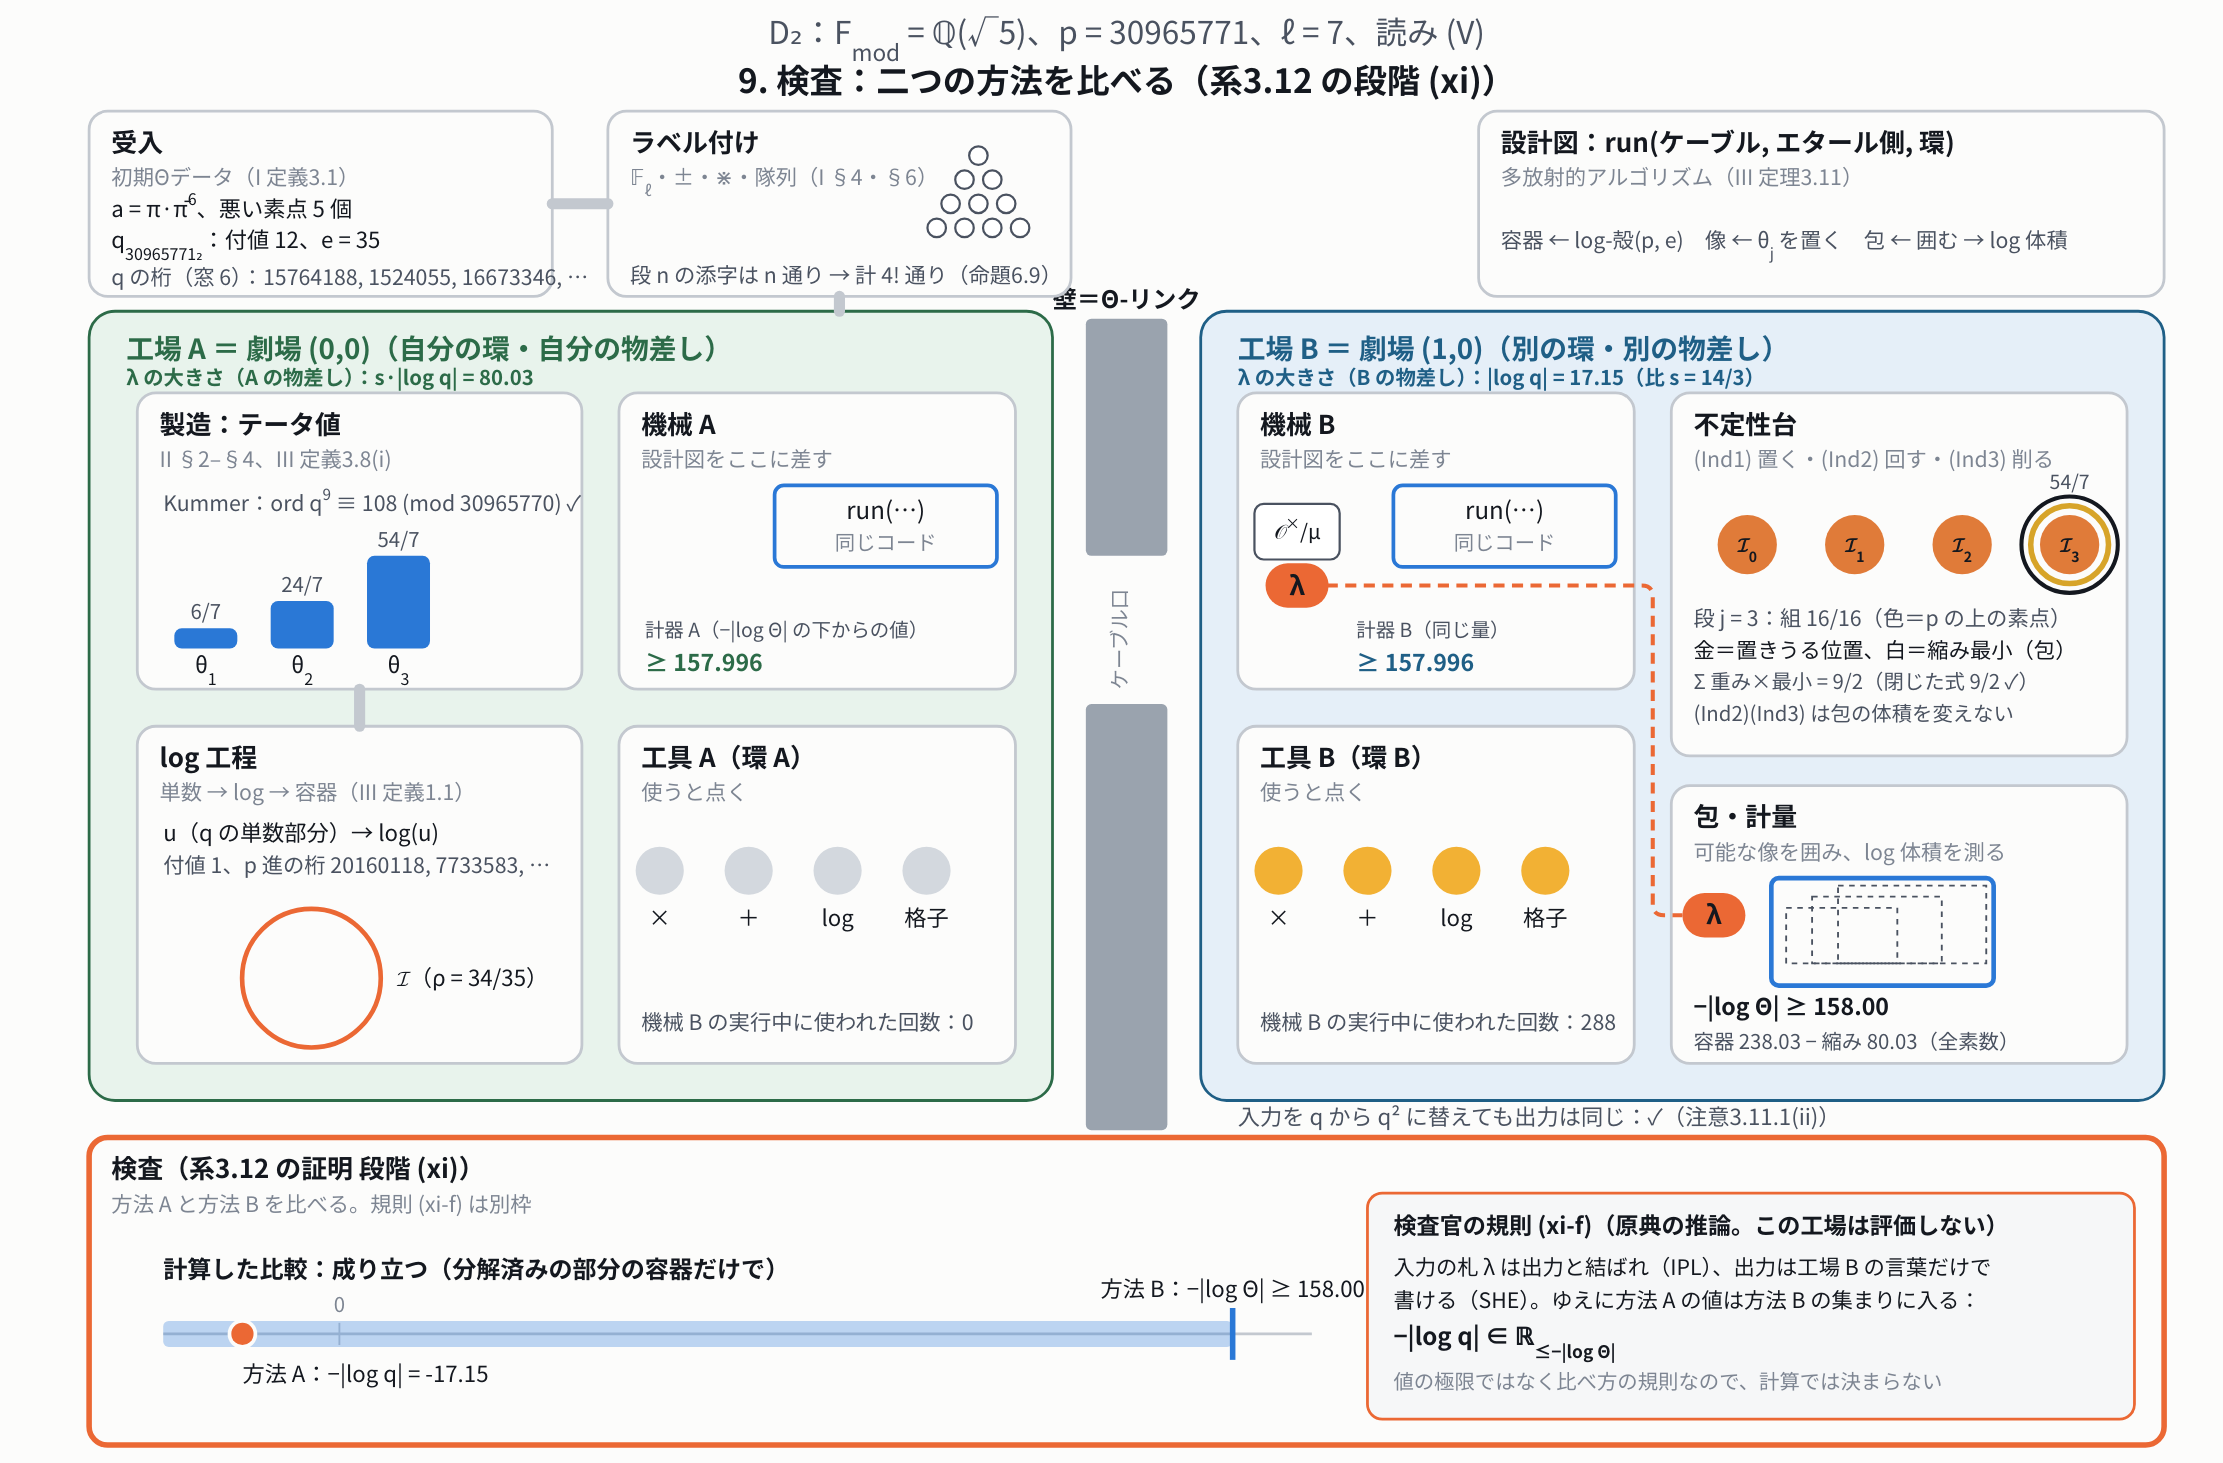
\includegraphics[width=0.86\textheight]{fig/fig1.png}
\caption{The factory tab for $D_2$ in reading (V), at the inspection step (labels in Japanese). Left: hall~A, the
theater $(0,0)$; right: hall~B, the theater $(1,0)$; between them the wall (the $\Theta$-link) with the slot through
which the cable passes. The same algorithm \code{run($\cdots$)} is installed in both halls and gives the same lower
bound $157.996$ in both (APT). While machine~B ran, the ring operations of hall~A were used $0$ times and those of
hall~B $288$ times (SHE), and replacing the input $q$ by $q^2$ did not change the output. The dashed thread ties the
object $\lambda$ that passed the wall to the output (IPL). The indeterminacy table shows the capsule of label $3$;
the hull box shows $-|\log(\Th)|\ge158.00=238.03-80.03$. At the bottom, the two numbers of Step~(xi) on a line,
and, in a separate box, the rule~(xi-f), which the page does not evaluate.}\label{fig:factory}
\end{sidewaysfigure}

\begin{figure}[p]
\centering
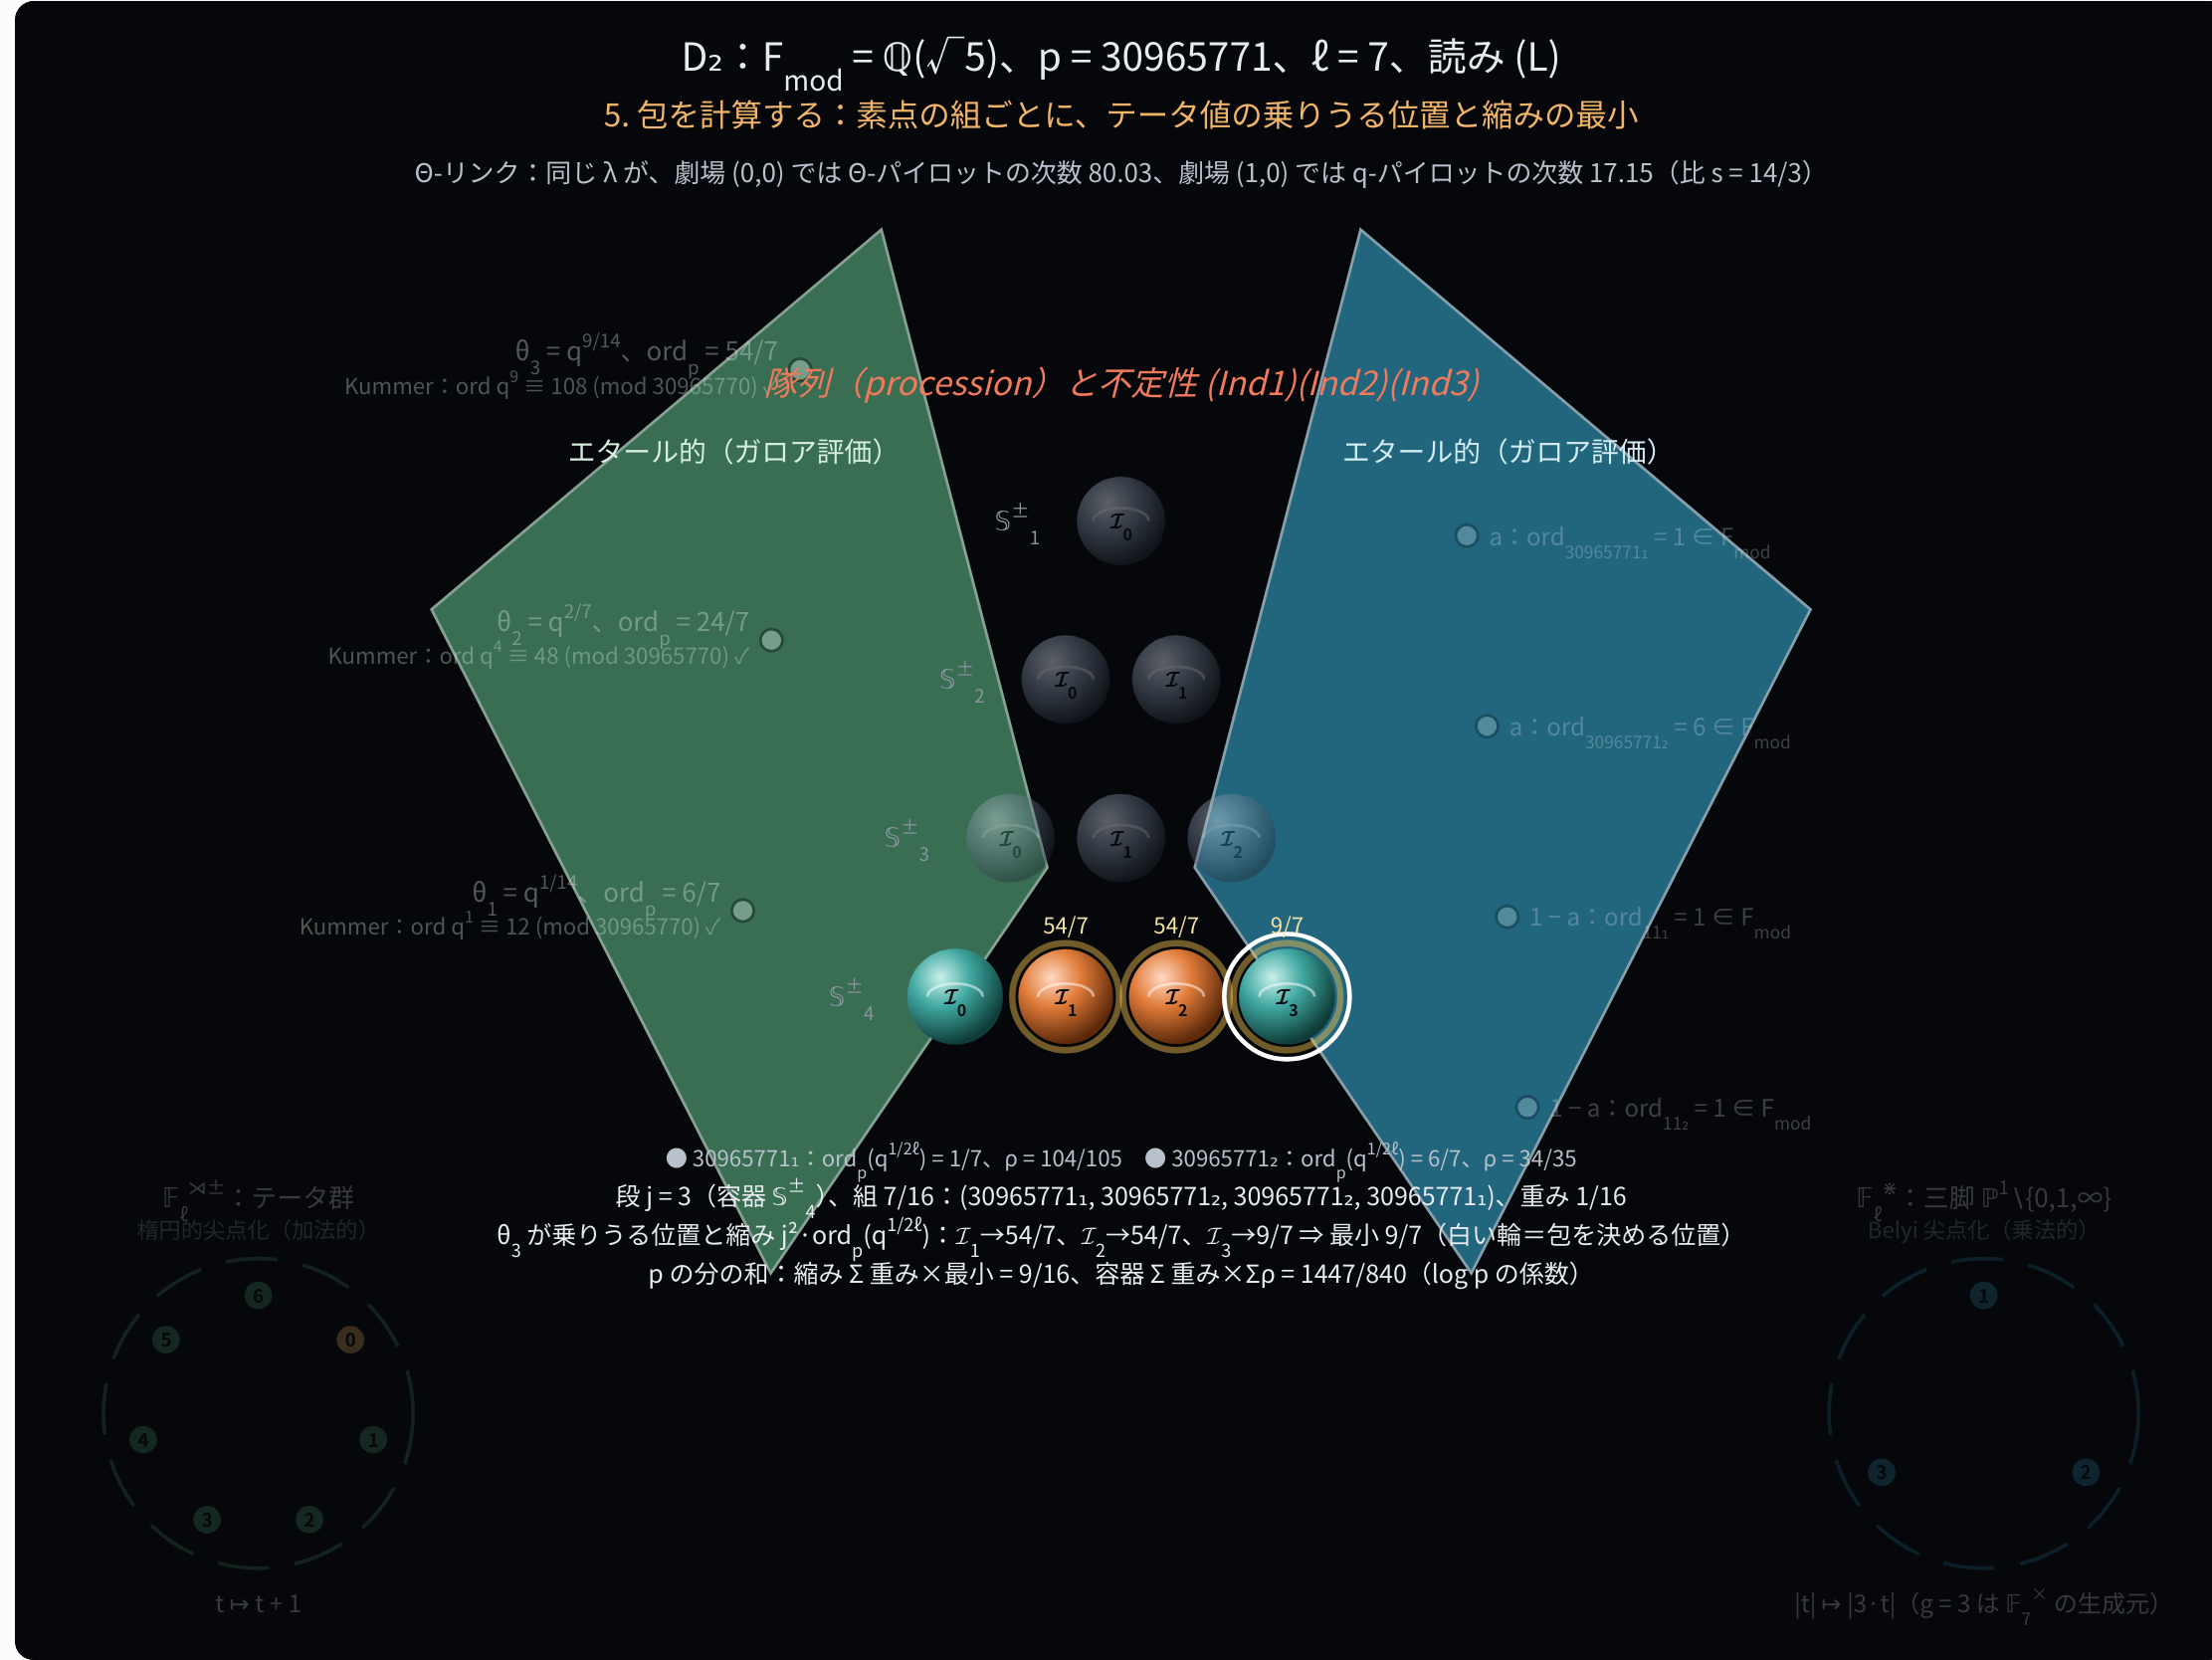
\includegraphics[width=0.92\textwidth]{fig/fig2.png}
\caption{The animation tab for $D_2$ in reading (L), during the enumeration of the capsule of label $3$ (labels in
Japanese). The factors $\cI_0,\dots,\cI_3$ are coloured by the place above $p$ in the current tuple, the seventh of
sixteen, of weight $1/16$. Gold rings mark the positions where the theta value may be placed in this reading, with
the shrinkage $j^2\ord_p(\qq_{v_t})$ above them ($54/7$, $54/7$, $9/7$); the white ring marks the least shrinkage,
which determines the hull. The running sums at the bottom are checked against the closed form at the end of the
capsule. The composition follows~\cite{Farcot}.}\label{fig:anim}
\end{figure}

\subsection{The toys of Remark 3.11.1}\label{sec:toys}
Remark~3.11.1(vi)--(viii) of~\cite{IUT3} illustrates IPL and SHE by naive constructions, which the program runs in
the same frame, at one place $w$ of $\Vbad$ and with $\lambda=2$. The naive $\Theta$-link $q\mapsto q^\lambda$
within one ring runs, with SHE holding tautologically, but links nothing (no analogue of IPL). With distinct labels
${}^\dagger R$ and ${}^\ddagger R$ the program cannot compute the comparison and raises the type error of
Section~\ref{sec:theaters}; Remark~3.11.1(vii) says that it is ``by no means clear, at least in any a priori sense, how
to `compute' the relationship'' between the two arithmetic holomorphic structures. With the forced identification of the two ring structures the output is the trivial
multiradial representation $\{\qq^{\lambda^n}\}_{n\in\Z}$; in the window $|n|\le W$ the upper bound of the possible
log-volumes is $-\lambda^{-W}c_wr_w\log p_w$, which tends to $0$, so the representation says nothing about
log-volumes, as Remark~3.11.1(viii) explains.

\section{What is computed, given and chosen}\label{sec:limits}
\paragraph{Computed.} The places, valuations and Tate parameters of the curve; the conditions of Definition~3.1 that
are decidable from them; the log-shell radii, with a check of the series; the Kummer read-outs; the containers,
possible images, hulls and log-volumes, exactly, in the first model of (Ind2) of Section~\ref{sec:algo}, and in the
second model exactly at the small places and as an interval elsewhere; the comparison of Step~(xi); the gap between
the two models; the toys.

\paragraph{Given.} That the theta values are $\qq^{\,j^2}$ up to roots of unity, from the theory of the \'etale theta
function as used in~\cite{IUT2}; the formula for $e$ of~\cite{Cat} at places other than those above $p$; the
log-volume formula for the hull of a tensor packet of~\cite{LANAiut}; the closed form of the hull in the second model
of (Ind2), proved on paper in~\cite{Gap}; the archimedean container
of~\cite[Thm.~1.10, proof, Step~(vii)]{IUT4}; the conditions of Definition~3.1 that the program does not check, such
as the image of Galois containing $\mathrm{SL}_2(\F_\ell)$, which are established in~\cite{Cat} and the sources cited
there.

\paragraph{Chosen.} The reading (Section~\ref{sec:readings}); the set $\Vbad$, which leaves out the places above $3$
and $5$ (Section~\ref{sec:data}); the places above $2,3,5,\ell$, whose contributions are set to $0$.

\paragraph{Limitations.} The anabelian reconstructions are not implemented: the theaters are given as typed copies of
fields, not reconstructed from groups, and the Kummer read-out is a round trip. The records of APT and SHE hold by
construction. The group of (Ind2) of the source is not modelled; by~\cite{LANAiut}, the two models bracket it. In
the second model, $\kappa_v(\theta)$ at the places that are not small is only bracketed, since the program does not
compute the log-shells as lattices in $K_v$, nor the unit parts of the theta values at places other than those
above $p$.
The model measures the theta values by their valuations in a container shared by the two columns; this is the
bookkeeping of the proof of Theorem~1.10 of~\cite{IUT4}, and the one in which the comparison takes the form of a
height inequality. A reader who holds that the output of the algorithm must be measured in another way will not find
that view implemented here. The inference~(xi-f) is not evaluated.

\section{Related work}\label{sec:related}
The toolkit \texttt{motizukipdf} of D.~Richards~\cite{Richards}, published in October 2026, turns the objects of
IUT~I--IV, of~\cite{EssLgc} and of related papers into C data types with validators, a registry of 73 processes, a
terminal interface, a web application that runs the C code in the browser, and a Lean port. Its coverage is far broader
than ours. Its data model lets a $\Theta$-link share the unit groups but never the ring structures (in its Lean port,
\nolinkurl{wellFormed_not_ring}), which is the first design rule of this note, and records (Ind1) as the $(j+1)!$
permutations of tensor factors. Its initial $\Theta$-data are generated from abc triples via Frey curves over $\Q$, or
synthetically; the conditions of Definition~3.1 that can be decided from numbers are checked, and the others are
recorded as asserted flags. Its log-volume report for Corollary~3.12 uses the explicit constant
of~\cite[Thm.~1.10]{IUT4} and a leading-term estimate of the hull. With this estimate its process \texttt{Fuzzify}
widens the $\Theta$-pilot to an interval and reports whether the interval contains $-|\log(\qq)|$, a numerical form of
the comparison of Step~(xi) in the terms of~\cite[\S3.10]{EssLgc}. Its arithmetic is in 64-bit integers and floating
point; by design, the Tate parameter enters through its valuation and the Kummer isomorphisms as recorded properties
(its data model tracks what is identified with what, not the reconstructions). Its Lean port follows the main strategy of~\cite{Formal}: it proves IPL
(\nolinkurl{mltAlgo_IPL}) and APT (\nolinkurl{dsc_APT}) for its model, defines SHE as an operation, and derives from
the comparison in the common container, left as a hypothesis, the bound $|\log(\qq)|\le H/(N-1)$
(\nolinkurl{corThreeTwelve_of_thmThreeElevenFive}), with $H$ its estimate of the hull term and $N=\ell(\ell+1)/12$:
the form of our comparison in reading (V). The present program was
written independently; it differs in using verified explicit data whose field of moduli is not $\Q$, in integers of
arbitrary size, with the Tate parameters computed $p$-adically and a Kummer read-out of the theta values (a round
trip, Section~\ref{sec:kummer}); in computing the hull of the union of the possible images exactly, for three
readings; in its windows; in running the toys of Remark~3.11.1(vi)--(viii) in the same frame as the algorithm; and in
recording IPL, SHE and APT as the execution of one program on numbers.

The analysis of the step from Theorem~3.11 to Corollary~3.12 by the LANA project~\cite{LANA} and its Lean
repository~\cite{LANAiut} underlies Sections~\ref{sec:readings}, \ref{sec:algo} and~\ref{sec:xi}: the log-volume of the
hull of a tensor packet of log-shells, the readings of IUT~IV and the literal reading together with the minimum
versus the average, and the equivalence, in its models, of Step~(xi) with an inequality of the form considered by
Scholze and Stix~\cite{SS}. Its file \nolinkurl{Iut/WallEquiv/Gap.lean} reduces the difference between this
inequality and its variant of Corollary~3.12 to (Ind2)-terms and leaves their value open; the author's
note~\cite{Gap} determines them, and Section~\ref{sec:algo} uses its closed form. Mochizuki's report~\cite{Formal} describes the formalization of the step from
Theorem~3.11 to Corollary~3.12 in Lean as a means of communicating the logical structure of the theory, and names IPL
and APT among its central aspects. The permutations of tensor factors in (Ind1) are discussed
in~\cite[\S4]{DH1} and \cite[\S6.2, footnote~7]{DH}. Explicit initial $\Theta$-data over $\Q$ are given
in~\cite[\S2.10]{DH1} and~\cite{Zhou1,Zhou2}, and explicit estimates in~\cite{MFHMP}. Expositions of the theory
include~\cite{Hoshi1,Hoshi2,Yamashita}. A different loss in the hull of a tensor packet, from boxing the integral
structure, is studied in~\cite{Zeng}; the question of the source of $\lambda=\ord(q^{j^2})$ in Step~(v), which the
program takes as given (Section~\ref{sec:limits}), is raised in~\cite{Takkun}. The data used here and their local
invariants are those of the author's catalogue~\cite{Cat}, which collects data from~\cite{First,Second,Note}; its
\S5 checks the comparison in reading (V) for $D_2$ with a lower bound for the container, and Table~\ref{tab:results}
extends this to all seven data.

\section*{Use of generative AI}
Generative AI tools (large language models) were used extensively in this work, under the author's direction, in
writing the program and the web page, in the computations and in the writing. The author takes full responsibility
for the contents of this note.

\appendix
\section{Reproducing the results}\label{app:repro}
The program is a single Python file (Python~3.10 or later with \texttt{sympy}). The commands
\begin{verbatim}
python3 iut_compute.py --all --reading V     # also L and L0
python3 iut_compute.py --data D2 --toys
python3 iut_compute.py --windows --data D211
python3 iut_compute.py --export-json run_data.json
\end{verbatim}
print the steps for all data, the toys, the windows, and the data block of the page. Each run of \texttt{-{}-all} takes
about fifteen seconds, and the export a little over a minute. Both models of (Ind2) are printed in every run. The recorded outputs are in the supplement, with the page and checksums.
The output of the program is in Japanese.

\section{The code and the source}\label{app:map}
\begin{center}\small
\begin{tabular}{>{\raggedright\arraybackslash}p{5.6cm}>{\raggedright\arraybackslash}p{8.4cm}}
\toprule
source & code\\
\midrule
IUT I, Definition 3.1; Example 3.2(iv) & \code{InitialThetaData}, \code{checks}, \code{table1\_check}\\
IUT I, \S\S4, 6; Propositions 6.8, 6.9 & \code{Labels}; the procession counts of the page\\
Hodge theaters & \code{Theater} (typed copies), \code{Elem}, \code{Lattice}\\
IUT I, Corollary 3.7; IUT III, Definition 3.8 & \code{theta\_link}, \code{Cable}, \code{ValuePart}\\
IUT III, Definition 1.1 & \code{padic\_log\_unit}, \code{log\_shell\_radius}, \code{LogShell.verify}\\
Kummer theory & \code{kummer\_recover}\\
IUT III, Theorem 3.11; Remark 3.11.1 & \code{IUTAlgorithm.run}, \code{placements}, \code{run\_with\_record}\\
(Ind2): the two models; \cite[Thms.~3.2, 3.3]{Gap}; IUT IV, Proposition 1.2(i) & \code{IUTAlgorithm(ind2=...)},
\code{kappa\_range}, \code{log\_shell\_ab}, \code{log\_shell\_inner}\\
IUT III, Corollary 3.12, Step (xi) & \code{integrate}\\
IUT III, Remark 3.11.1(vi)--(viii) & \code{NaiveLink}, \code{DistinctLabels}, \code{ForcedIdentification}\\
\bottomrule
\end{tabular}
\end{center}

\begin{thebibliography}{Yamashita}

\bibitem[Cat]{Cat}
Toshihisa Urahigashi, \emph{Explicit initial $\Theta$-data and the two readings of Step~(v) of IUT~IV,
Theorem~1.10: a catalogue}, version 1.0.0, Zenodo, 2 November 2026,
\href{https://doi.org/10.5281/zenodo.23870448}{doi:10.5281/zenodo.23870448}.

\bibitem[DH]{DH}
Taylor Dupuy and Anton Hilado, \emph{Probabilistic {S}zpiro, baby {S}zpiro, and explicit {S}zpiro from
{M}ochizuki's {C}orollary 3.12}, 2020, arXiv:2004.13108v2 [math.NT].

\bibitem[DH1]{DH1}
Taylor Dupuy and Anton Hilado, \emph{The statement of {M}ochizuki's {C}orollary 3.12, initial theta data, and
the first two indeterminacies}, 2020, arXiv:2004.13228 [math.NT]; \S4 refers to version~1, \S2.10 to version~2
(2025).

\bibitem[EssLgc]{EssLgc}
Shinichi Mochizuki, \emph{On the essential logical structure of inter-universal {T}eichm\"uller theory in
terms of logical {AND} ``$\wedge$''/logical {OR} ``$\vee$'' relations: report on the occasion of the
publication of the four main papers on inter-universal {T}eichm\"uller theory}, RIMS Preprint 1968, November
2022.

\bibitem[Farcot]{Farcot}
Etienne Farcot, \emph{The Multiradial Representation of Inter-universal Teichm\"uller Theory}, animation made
from the specifications of Shinichi Mochizuki and suggestions of Ivan Fesenko, licensed under CC BY 4.0,
\url{https://www.kurims.kyoto-u.ac.jp/~motizuki/research-english.html} (consulted 2 November 2026).

\bibitem[First]{First}
Toshihisa Urahigashi, \emph{An explicit initial $\Theta$-datum with mixed reduction at a split prime},
version 0.1.7, Zenodo, \href{https://doi.org/10.5281/zenodo.22537342}{doi:10.5281/zenodo.22537342}.

\bibitem[Formal]{Formal}
Shinichi Mochizuki, \emph{On the formalization of {IUT}: a preliminary progress report [joint work in progress
with {Y.~Hoshi}, {G.~Yamashita}, {Y.~Yang}, \dots]}, April 2026.

\bibitem[Gap]{Gap}
Toshihisa Urahigashi, \emph{The gap between the two walls is positive: a closed form for the (Ind2)-terms of
lana-agents/iut}, version 1.0.0, Zenodo, 5 November 2026,
\href{https://doi.org/10.5281/zenodo.23954194}{doi:10.5281/zenodo.23954194}.

\bibitem[Hoshi1]{Hoshi1}
Yuichiro Hoshi, \emph{Introduction to inter-universal {T}eichm\"uller theory} (in Japanese), RIMS
K\^oky\^uroku Bessatsu \textbf{B76} (2019), 79--183.

\bibitem[Hoshi2]{Hoshi2}
Yuichiro Hoshi, \emph{Introduction to inter-universal {T}eichm\"uller theory, continued} (in Japanese), RIMS
K\^oky\^uroku Bessatsu \textbf{B72} (2018), 209--307.

\bibitem[IUT1]{IUT1}
Shinichi Mochizuki, \emph{Inter-universal {T}eichm\"uller theory {I}: construction of {H}odge theaters},
Publ. Res. Inst. Math. Sci. \textbf{57} (2021), 3--207.

\bibitem[IUT2]{IUT2}
Shinichi Mochizuki, \emph{Inter-universal {T}eichm\"uller theory {II}: {H}odge--{A}rakelov-theoretic
evaluation}, Publ. Res. Inst. Math. Sci. \textbf{57} (2021), 209--401.

\bibitem[IUT3]{IUT3}
Shinichi Mochizuki, \emph{Inter-universal {T}eichm\"uller theory {III}: canonical splittings of the
log-theta-lattice}, Publ. Res. Inst. Math. Sci. \textbf{57} (2021), 403--626.

\bibitem[IUT4]{IUT4}
Shinichi Mochizuki, \emph{Inter-universal {T}eichm\"uller theory {IV}: log-volume computations and
set-theoretic foundations}, Publ. Res. Inst. Math. Sci. \textbf{57} (2021), 627--723.

\bibitem[LANA]{LANA}
Project LANA, \emph{Project LANA interim report on IUT theory}, last updated 20 July 2026.

\bibitem[LANA-iut]{LANAiut}
lana-agents, \emph{iut}, Lean repository, \url{https://github.com/lana-agents/iut}, consulted at commit
\texttt{553076a} (3 November 2026); the files cited are unchanged since commit \texttt{ecb3c86} (1 November 2026).

\bibitem[MFHMP]{MFHMP}
Shinichi Mochizuki, Ivan Fesenko, Yuichiro Hoshi, Arata Minamide, and Wojciech Porowski, \emph{Explicit
estimates in inter-universal {T}eichm\"uller theory}, Kodai Math. J. \textbf{45} (2022), no.~2, 175--236.

\bibitem[Note]{Note}
Toshihisa Urahigashi, \emph{A local non-containment in Step~(v) of {IUT}~{IV}, Theorem~1.10}, version 3.0.0,
Zenodo, 1 November 2026, \href{https://doi.org/10.5281/zenodo.23852752}{doi:10.5281/zenodo.23852752}.

\bibitem[Richards]{Richards}
David Richards, \emph{motizukipdf---{M}ochizuki's papers, plus a toolkit for the data types of {IUT}}, GitHub
repository \url{https://github.com/oneman/motizukipdf}, consulted at commit \texttt{2665db1} (30 October 2026).

\bibitem[Second]{Second}
Toshihisa Urahigashi, \emph{An initial $\Theta$-datum over an imaginary quadratic field, and numerical values
of the local quantities of inter-universal {T}eichm\"uller theory~{IV}}, version 1.0.5, Zenodo,
\href{https://doi.org/10.5281/zenodo.22601333}{doi:10.5281/zenodo.22601333}.

\bibitem[SS]{SS}
Peter Scholze and Jakob Stix, \emph{Why abc is still a conjecture}, manuscript, 2018.

\bibitem[Takkun]{Takkun}
Takkun-kohinata, \emph{IUT\_LEAN}, GitHub repository, \url{https://github.com/Takkun-kohinata/IUT_LEAN} (July 2026).

\bibitem[Yamashita]{Yamashita}
Go Yamashita, \emph{A proof of the abc conjecture after {M}ochizuki}, preprint, RIMS, Kyoto University.

\bibitem[Zeng]{Zeng}
Chunping Zeng, \emph{An integral-structure inflation in the hull operation of {IUT} {C}orollary 3.12}, Zenodo, 30
October 2026, \href{https://doi.org/10.5281/zenodo.23811410}{doi:10.5281/zenodo.23811410}.

\bibitem[Zhou1]{Zhou1}
Zhong-Peng Zhou, \emph{The inter-universal {T}eichm\"uller theory and new {D}iophantine results over the
rational numbers.~{I}}, arXiv:2503.14510 [math.NT], 2025.

\bibitem[Zhou2]{Zhou2}
Zhong-Peng Zhou, \emph{The inter-universal {T}eichm\"uller theory and new {D}iophantine results over
rational numbers.~{II}}, arXiv:2510.05448 [math.NT], 2025.

\end{thebibliography}
\end{document}
